This chapter covers the architecture and design of the system.
\section{General architecture}
In this section the general architecture of the \gls{theresa} system is described.
The idea for the new system is to reuse the concept of the already existing sampling system \gls{kapture}, which is using four \glspl{adc}, and expanding it to 16. Therefore, also the architecture of the latter is explained briefly.

\newpage
\subsection{New System THERESA}
In principle, the new system has the same structure, as \gls{kapture}. Notable differences are firstly the number of \glspl{adc}, which is increased up to 16. Secondly, the latter are not located on the daughter card anymore, but inside the Xilinx Zynq UltraScale+ RFSoC ZU49DR on the ZCU216 Evaluation Kit on which the front-end card is mounted.
%todo On THE xyz board? do we know what this is at this point?





\subsection{Requirements}
\paragraph{Interleaving}
The necessary step size for the delay chips, when using 16 ADC@\SI{2}{\giga \sample \per \second} in time-interleaving mode, is: $\frac{\SI{2}{\giga \sample \per \second}}{16} = \SI{31}{\pico \second}$
However, providing individual clocks to the ADCs is not possible on the ZCU216 card. ADCs are grouped together into tiles, each tile containing four converters. One single reference clock signal is propagated to all tiles. Sampling clock is adjusted at each tile individually, however this clocking signal is the same for all of the four converters in the tile.

Clock to THA: \SI{500}{\mega \hertz}

Total Hold time: \SI{1}{\nano \second}

$\rightarrow$ Step size for delay:
\begin{equation}
	\frac{\SI{1}{\nano \second}}{16 \, \text{channels}} = \SI{62.5}{\pico \second}
\end{equation}

\begin{figure}[tbh]
\centering
\tikzexternaldisable
\begin{tikztimingtable}
  TH1 & 1L 8H N(A1) 8H 16L \\
  TH2 & 2L 16H 15L \\
  TH3 & 3L 16H 14L \\
  TH4 & 4L 5H N(B1) 11H 13L \\
  \\
  TH5 & 5L 16H 12L \\
  TH6 & 6L 16H 11L \\
  TH7 & 7L 16H 10L \\
  TH8 & 8L 16H 9L \\
  \\
  TH9 & 9L 16H 8L \\
  TH10 & 10L 16H 7L \\
  TH11 & 11L 16H 6L \\
  TH12 & 12L 16H 5L \\
  \\
  TH13 & 13L 16H 4L \\
  TH14 & 14L 16H 3L \\
  TH15 & 15L 16H 2L \\
  TH16 & 16L 16H 1L \\
\extracode
 \tablerules
 \begin{pgfonlayer}{background}
 \draw [help lines, dashed] (A1) -- (B1);
 \end{pgfonlayer}
\end{tikztimingtable}
\tikzexternalenable
\caption{Track-And-Hold Timing diagram}
\label{fig:THA}
\end{figure}
%todo what does the dashed line show?




\paragraph{Data Rate}

ADC samples \@ \SI{2.5}{\giga \hertz} with 14-bit resolution.

\paragraph{Visualization/GUI}
\newpage
\section{Design of the front-end card}
In this section, the design of the front-end card is covered.



\newpage
\section{PCB-Layout}


  
\newpage
\section{Firmware}
\subsection{General Design}
\subsubsection{Firmware for Front-End Card}
\paragraph{Clocking}
\paragraph{SPI-Interface}
\subsubsection{Data Capture}
\begin{figure}[H]
	\centering
	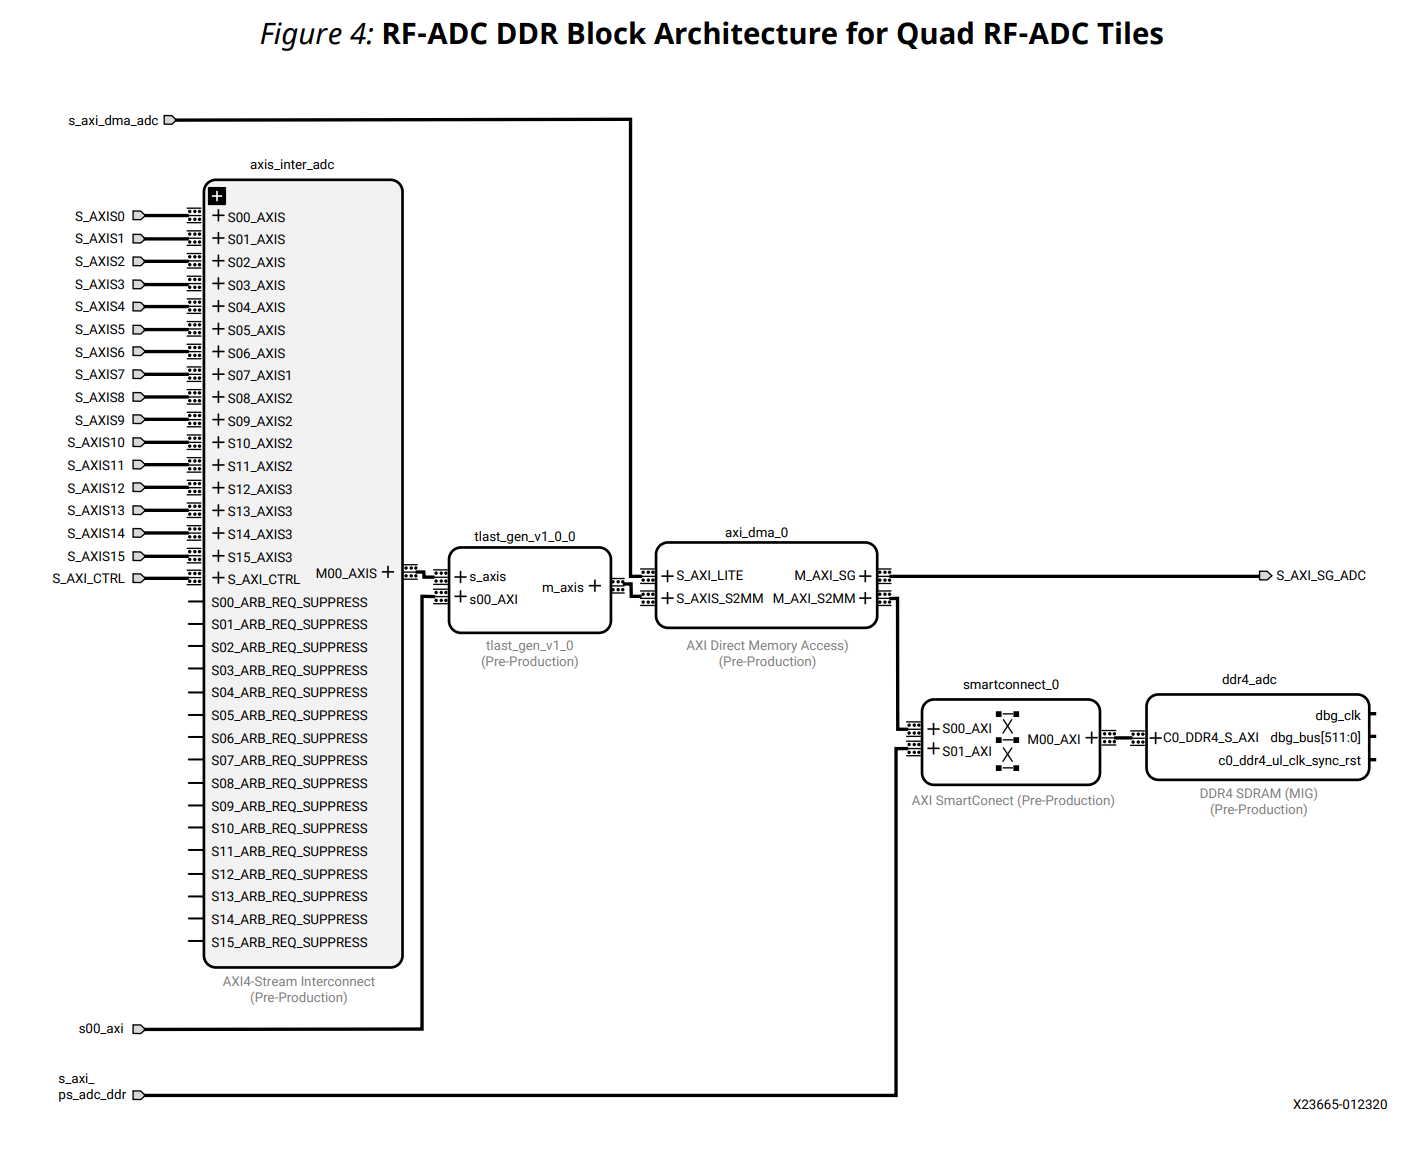
\includegraphics[width = 0.8\textwidth]{chap/04-work/img/adc_cap}
	\caption{Placeholder}
	\label{fig:adccap}
\end{figure}

\subsubsection{Visualization}





